\documentclass{article}

\usepackage[a4paper, margin=1in]{geometry}

\usepackage{graphicx}
\graphicspath{ {./images/} }

\title{Informação Profissional em Ciência da Computação:\\
  Arquitetura de Computadores}
\author{Carlos Eduardo Gallo Filho \\
  Caio \\
  Pedro}

\date{\today}

\begin{document}

\maketitle

\section{Introdução}
\subsection{Arquitetura e Organização}
\subsection{Estruturas e Funções}
\subsubsection{Múltiplos núcleos}
\subsubsection{Estrutura interna do núcleo}

\section{Evolução histórica}
\subsection{Primeira geração: Arquitetura de Von Neumann}
A primeira geração de computadores é conhecida pelo uso das válvulas para
representar os elementos lógicos digitais e a memória. E também, o
\textit{conceito de programa armazenado}, atribuída ao matemático John Von
Neumann, que surgiu para a construção do computador EDVAC (Eletronic Discrete
Variable Computer), mas foi principalmente discutido no desenvolvimento do
computador IAS, o qual é um protótipo para quase todos os computadores de
propósito geral de hoje em dia.

\begin{figure}[h]
  \centering
  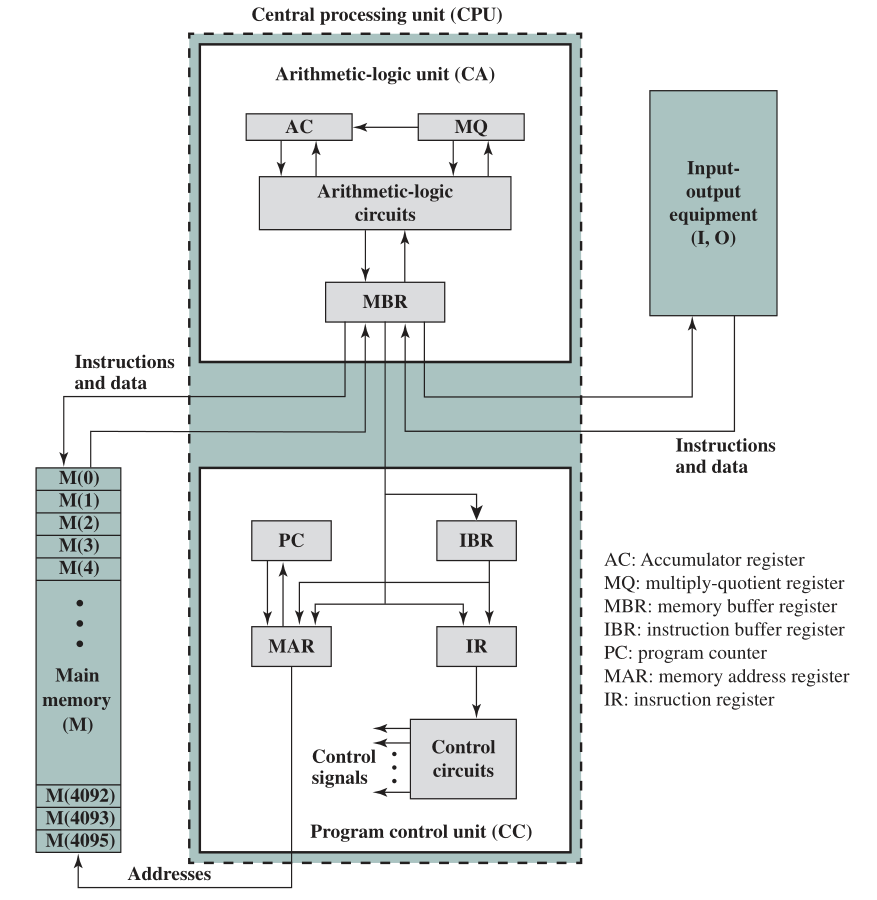
\includegraphics[width=0.7\textwidth]{ias.png}
  \caption{Estrutura do IAS.}
\end{figure}

Para se explicar a estrutura do IAS, deve-se atentar a 5 partes principais:

\begin{enumerate}
\item Um computador terá de ser capaz de executar as
  operações elementares básicas (adição, subtração, multiplicação,
  divisão). Normalmente, para essas funções são criadas unidades
  específicas para tais, comportadas em uma unidade maior
  centralizadora denominada CA ou unidade lógica e aritmética.

\item Um computador terá de ser capaz de dar sequenciamento adequado as
  suas operações, instruções e as instruções de controle (comandos que
  regem o próprio sequenciamento do computador). Á essas undides é
  denomiada uma unidade central chamada CC ou controle central.

  As partes 1) e 2) juntas são chamadas de C. 

\item Um computador terá a necessidade de processar sequências longas de
  operações, que, geralmente, não conseguem ser efetuadas em uma única
  leva de comandos. Logo, requer-se uma unidade que armazene dados por
  períodos duráveis para resolver problemas mais complexos, como
  cálculos.

  Essa unidade é denominada M ou memória.

  Analogamente ao funcionamento do corpo humano, essas três partes podem
  ser comparadas a parte cognitiva do corpo. Ou seja, a unidade lógica e
  aritmética, o controle central e a memória são o conjunto pensante do
  computador. Mas, assim como o corpo humano, se faz necessário a
  comunicação com o mundo externo, tal é feito por um canal denominado
  meio de gravação de sáida do dispositivo ou R, de modo que as últimas
  duas partes interagem com esse canal para satisfazer a necessidade de
  interação com o externo. 

\item A parte de entrada do meio R, a qual deve transferir as informações
  desse para dentro de M e C é chamada de entrada ou I. É de boa prática a
  entrada passar os dados para dentro de M e nunca diretamenta para C. 

\item Similarmente, a parte de saída do meio R, a qual deve transferir as
  informações de M e C para o meio R, é chamada de saída ou O. É de boa
  prática, também, a saída passar de M para R, assim, nunca diretamente
  por C. 
\end{enumerate}

Assim, resumidamente, temos a memória principal, que armazena dados e
instruções; a unidade lógica e aritmética (ALU), que opera os binários; a
unidade de controle, que interpreta e executa instruções e, por fim, o
equipmaneto de saída (E/S), que conecta o meio interno ao meio externo do
computador.

\subsubsection{Endereçamento de memória}

\subsection{Segunda geração: Transístores}
\subsection{Terceira geração: Circuitos Integrados}
\subsection{Gerações posteriores}

\section{Aplicações} 
As subseções a seguir trazem algumas aplicações da arquitetura de computadores.
\subsection{Paradigmas de arquitetura}

\subsubsection{CISC}
O paradigma de arquitetura CISC (\textit{Complex Instruction Set
  Computer}) denotam uma escolha de projeto na qual o conjunto das
instruções utilizadas são projetadas para a execução de um conjunto de
operações de baixo nível, envolvendo por exemplo, operações
aritméticas juntas de uma escrita na memória, tudo em uma mesma
instrução.

Uma notória vantagem do uso do paradigma CISC se dá por facilitar a construção
de compiladores e a programação em baixo nível, pois as instruções fornecem um
pequeno nível de abstração. Além disso, por implementar as instruções a comuns
nível de \texti{hardware}, o consumo de memória, tempo de execução e tamanho
dos programas costumam ser menores. Uma desvantagem direta ao paradigma é o
fato do projeto do hardware se tornar muito mais trabalhoso e complexo, além de
necessitar maior quantidade de componentes, e por consequência, aumento de
calor.

\subsection{RISC}
Em contrapartida ao CISC, existe o paragima RISC (\textit{Reduced Instruction
  Set Computer}). Um projeto RISC tem como princípio implementar um pequeno
número mínimo de instruções simples, que em sua maioria são executadas em
apenas um cíclo de máquina.

Como esperado, processadores RISCs são mais fáceis de serem implementados e
produzidos, gastando menor quantidade de componentes e melhorando a eficiência
térmica, além de facilitar a implementação do \textit{pipelining} a nível do
código de máquina. Como desvantagem, sua programação de baixo nível é mais
complexa, bem como a construção de compiladores, o que implica uma má
implementação a nível de software ser mais danosa.

\subsection{Arquitetura x86} 
A arquitetura de processadores x86 foi concebida pela intel e é o exemplar mais
popular do tipo CISC, trazendo muitos princípios de \textit{design} que só
existiam até então em \textit{mainframes}. A arquitetura teve seu surgimento
junto ao processador 8086 em 1978, que foi introduzido como uma extensão de 16
bits ao famoso 8080, primeiro microprocessador de propósito geral.

A linhagem de processadores x86 continou a evoluir, levando ao aparecimento do
80286, 80386 e 80486, cada qual incrementando novas instruções na arquitetura,
além de melhorar aspectos de organização utilizando a rápida evolução da
microeletrônica. O 80286 possibilitou a ampliação do número de memória
endereçável para 16 MB, ao invés de 1 MB que seu antecessor era capaz. Já o
80386 foi o primeiro processador de 32 bits, trazendo muitas melhorias em
comparação ao 80236, o que incluu o suporte a multitarefas. Sucessivamente,
o 80486 incrementou uma nova tecnologia de cache junto de uma avançada
\textit{pipelining} de instruções, além de também adicionar um coprocessador
para instruções matemáticas complexas.

Já entrando na quinta geração de processadores, surge o Pentium, que sucede o
80486 adicionando tecnologia superescalar, que é uma forma de paralelismo a
nível de instrução utilizando múltiplas unidades de execução. Seguindo para
o Pentium Pro, este continuou a implementação de tecnicas multiescalares,
incluindo análise do fluxo de dados, execução especulativa, entre outras.

Com os desktops se tornando cada vez mais comuns e novas necessidades surgindo,
levando ao aparecimento de instruções orientadas ao processamento de multimídia.

O Pentium II surge incorporando a tecnologia MMX da Intel no Pentium Pro. Em
seguida, o Pentium III trouxe muitas outras novas instruções de ponto flutuante,
que melhoravam muito a performance em algumas aplicações específicas. O ultimo
proessador da linha foi o Pentium 4, que apenas melhorou algumas tecnologias
utilizadas em seu antecessor.

Após a virada do século, o desenvolvimento de novos processadores acabou mudando
de rumo, quando foi alcançado limites práticos para o aumento do \textit{clock},
por exemplo. Como não era possível mais aproveitar os avanços da miniaturização
para melhorar a performance, os processadores passaram a serem multiplicados
em diferentes núcleos. O primeiro \textit{dual core} x86 foi o Intel Core.
Posteriormente o Intel Core foi extendido a 64 bits, surgindo posteriormente
variantes como o Core 2 Quad, com quatro núcelos. Outra tecnologia importante
adicionada à linha Core 2 foram as AVE, que possuiam instruções de grande
tamanho para processamento eficiente de vetores.

Por mais que a arquitetura x86 seja antiga, ela se mostrou em constante
evolução, o que inclui sempre a adição de novos recursos e instruções,
aproveitando os avanços da microeletrônica para mudanças na organização. Ainda
assim, processadores recentes possuem retrocompatibilidade com programas
antigos, devido ao fato da arquitetura ter evoluido sem alterar instruções já
existentes, o que colaborou para a manutenção da popularidade da arquitetura.

\subsection{Sistemas embarcados}
Sistemas embarcados são caracterizados pela combinação de
\textit{hardware} e \textit{software} utilizados em conjunto para
formar um sistema de propósito específico, em contraste aos
computadores de propósito geral abordados. Os tipos de sistemas
embarcados são dos mais variados, incluindo desde sistemas automotivos
até telefones celulares.

A organização de um sistema embarcado, como esperado, também difere à
de um sistema de propósito geral, o que inclui partes estritamente
planejadas para o ambiente de trabalho do sistema. Isso implica que no
geral, sistemas embarcados diferem muito entre si, e portanto são
difíceis de serem caracterizados de maneira genérica. No entanto,
algumas características comuns de sistemas embarcados podem ser
descritas:

\begin{figure}[h]
  \centering
  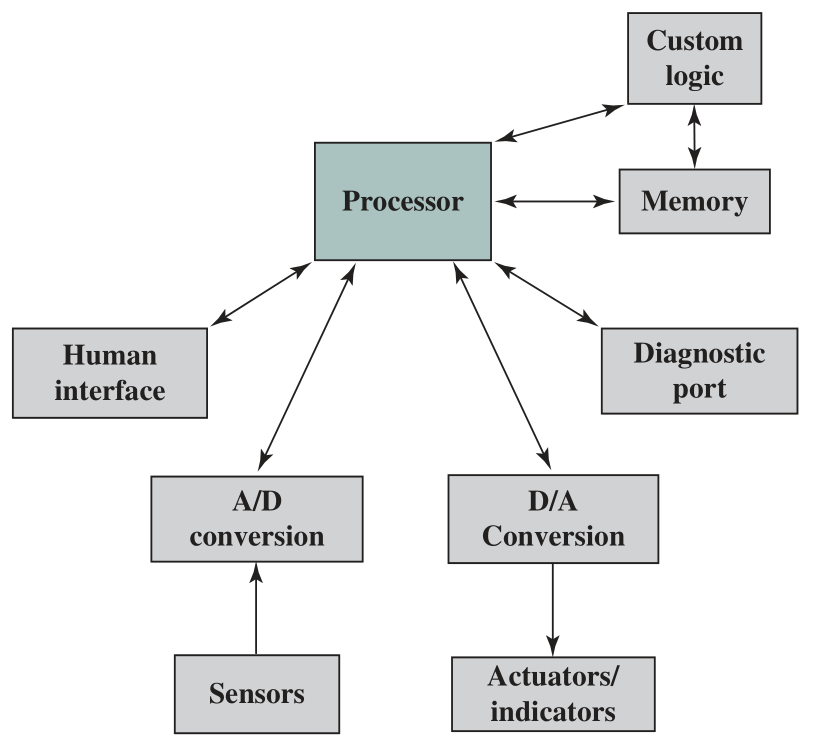
\includegraphics[width=0.4\textwidth]{embarcado.png}
  \caption{Possível organização de um sistema embarcado}
\end{figure}

\begin{itemize}
\item Possuem uma interface de comunicação com o ambiente,
  o que inclui sensores integrados.

\item A interface de usuário é simplificada, sendo até mesmo
  inexistente em alguns projetos.

\item A interface de depuração muitas vezes é utilizada para
  diagnostico do sistema controlado, não apenas do microcontrolador.

\item Uso de hardware especializado, incluindo até mesmo circuitos
  não digitais em alguns casos.

\item Software possui uma função e objetivo fixo e bem definido.

\item Eficiencia é de extrema importancia, o que inclui performance,
  baixo consumo de energia, espaço e consumo de memória.
\end{itemize}

Alguns sistemas embarcados complexos acabam incorporando processadores
de aplicação, capaz de executarem sistemas operacionais complexos, o
que inclui a adição da natureza de propósito geral aos
microcontroladores, ainda que em suma maioria estes possuam apenas um
processador dedicado.

\subsubsection{Microcontroladores}
Enquanto microprocessadores se beneficiaram dos avanços da
miniaturização de componentes aumentando seu conjunto de instruções,
memória e núcleos, os microcontroladores o usam para integrar todos os
outros componentes de um computador em um único chip, o que inclui
memória RAM, ROM, \textit{clock} e unidade de controle de entrada e
saída. Obviamente, os elementos de um microcontrolador são mais
simples, porém possuem alta eficiencia energética e baixíssimo custo.

\begin{figure}[h]
  \centering
  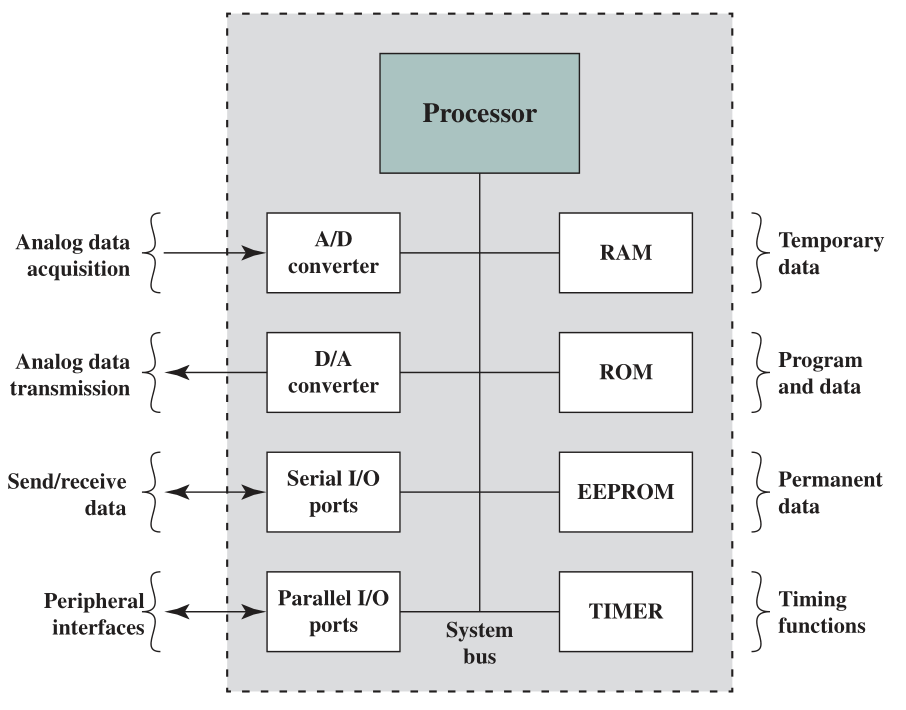
\includegraphics[width=0.6\textwidth]{uc.png}
  \caption{Organização típica de um microcontrolador}
\end{figure}

\subsubsection{Internet das Coisas (IoT)}
O termo IoT (\textit{Internet of Things}) é utilizado para denotar o
fenômeno de expansão da rede de comunicação entre dispositivos
embarcados "inteligentes". O fenômeno vem se tornando cada vez mais
popular e denota a inclusão de sistemas microcontrolados em objetos
dos mais variados tipos, como geladeira, lampadas e torradeiras. a IoT
é responsável pela integração dos possíveis objetos para formar um
grande sistema automatizável. Um exemplo clássico de IoT são os
sistemas de automação residencial.

Uma caraterística importante dos sistemas IoT é o caráter da conexão
dos seus principais dispositivos, definida por baixa largura de banda,
baixa repetição de captura e uso de dados.

\subsection{Arquitetura ARM} 

\subsection{Computação em Nuvem}

\end{document}
